\documentclass[../main.tex]{subfiles}
\begin{document}
\section{Policy implications}
\label{sec:policy_implications}
In this paper, we have identified the demographic transition as a significant contribution to the decline in the NRI in Denmark. The ageing of the Danish population also implies that the government faces the challenge of ensuring public pension system stability by adjusting expenditures to pension benefits. In this section, we analyze real-life pension system reforms suggested by the Danish government  - either through a reduction in the replacement rate, an increase in retirement age or a combination of both. This has different but significant implications for the NRI in Denmark within this model setup. 

We furthermore explore the idea of how historically low interest rates affect monetary policy instruments. We will focus on the limitations of conventional monetary policy and reflect on possibilities for unconventional monetary policy in low interest rate environments. 

\subsection{Pension system reforms}
\label{sec:pension_reform}
To impose realistic pensions system reforms, we change the budget constraint faced by the representative agent: 
\begin{equation}
    c_{j, t}+a_{j+1, t+1}=\left(1-\tau_{t}\right)\left[\left(1-\rho_{j, t}\right) w_{t} z_{j}+\rho_{j, t} \operatorname{pen}_{t}\right]+\pi_{j, t}+b e q_{t}+\left(1+r_{t}\right) a_{j, t}
    \label{eq:new_budget_constraint_pensions}
\end{equation}
$\rho_{j, t}$ can be interpreted as a fraction of time spent in retirement in a given year (or a fraction of a given cohort in retirement). It allows for a gradual exogenous increase in retirement age. Arguably, this is a somewhat more appropriate way than simply increasing the retirement age by one year at a time over the whole simulation period when using the original budget constraint (\ref{eq:budget_constraint_OG}). 

Furthermore, to illustrate the room for policy change by the government, we rewrite the government budget constraint (\ref{eq:government_budget_constraint_OG}) to:
\begin{equation}
    \left(1+\gamma_{t+1}\right) b_{t+1}^{y}-\left(1+r_{t}\right) b_{t}^{y}=g_{t}^{y}+\frac{1-\alpha}{u}\left[\left(1-\tau_{t}\right) \varrho_{t} d_{t}-\tau_{t}\right]
    \label{eq:government_budget_constraint_new}
\end{equation}
Where $d_{t}=\left(\sum_{j=J R}^{J} N_{j, t}\right) /\left(\sum_{j=1}^{J R-1} N_{j, t}\right)$ is the dependency ratio and $\gamma_t$ is the real growth rate of aggregate real GDP, $g_{t}^{y}$ and $b_{t}^{y}$ are the shares of public expenditure and public net debt in percent of GDP. From here we can directly see that the financial pressure to the public pension system can be alleviated by increasing the retirement age $JR$ (which automatically decreases the dependency ratio) or decreasing the replacement rate $\varrho_t$.

We base changes to the public pension system on proposed changes to the retirement age and replacement rate in Denmark, see table \ref{tab:replacement_rate} and \ref{tab:retirement_age}.

\begin{table}[H]
\centering
\caption{Pension system reforms, replacement rate}
\label{tab:replacement_rate}
\begin{threeparttable}
\begin{tabular}{llllll}
\hline
\textbf{2020} & \textbf{2030} & \textbf{2040} & \textbf{2050} & \textbf{2060} & \textbf{2070} \\ \hline
\multicolumn{1}{c}{42\%}        & \multicolumn{1}{c}{38\%}          & \multicolumn{1}{c}{36\%}          & \multicolumn{1}{c}{35\%}          & \multicolumn{1}{c}{35\%}          & \multicolumn{1}{c}{34\%}          \\ \hline
\end{tabular}
       \begin{tablenotes}
           \footnotesize Source: \textcite{pension_system_replacement_rate}
       \end{tablenotes} 
    \end{threeparttable}
\end{table}

\begin{table}[H]
\centering
\caption{Pension system reforms, retirement age}
\label{tab:retirement_age}
\begin{threeparttable}
\begin{tabular}{llllll}
\hline
\textbf{2020}          & \textbf{2030}          & \textbf{2040}          & \textbf{2050}          &
\textbf{2060}          & \textbf{2070}
          \\ \hline
\multicolumn{1}{c}{65} & \multicolumn{1}{c}{68} & \multicolumn{1}{c}{70} & \multicolumn{1}{c}{72} &
\multicolumn{1}{c}{73} & \multicolumn{1}{c}{74} \\ \hline
\end{tabular}
    \begin{tablenotes}
           \footnotesize Source: \textcite{Folkepension}
       \end{tablenotes} 
    \end{threeparttable}
\end{table}


Both pension system reforms help to ensure fiscal sustainability in the future as expenditures to gross old-age pensions are lowered (Figure \ref{fig:The_role_of_pension_system_reforms}\textcolor{blue}{C}). Nonetheless, these different changes to the pension system have vastly different implications for the NRI illustrated in Figure \ref{fig:The_role_of_pension_system_reforms}\textcolor{blue}{D}.

\begin{figure}[H]
    \centering
    \caption{The role of pension system reforms}
    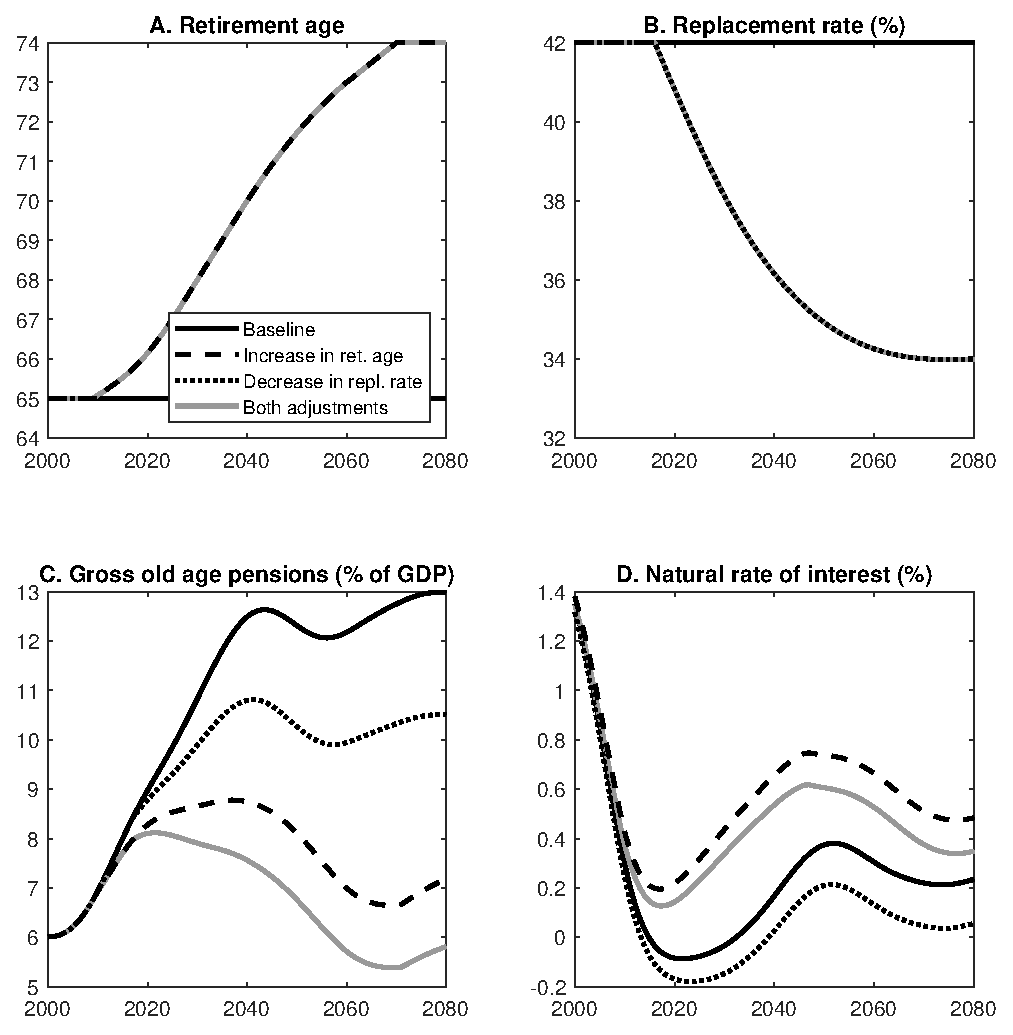
\includegraphics[scale=0.8]{Figures/Figure_10.eps}
    \label{fig:The_role_of_pension_system_reforms}
\end{figure}

The two effects on the pension system reforms illustrate opposite incentives to accumulate private savings to finance old-age consumption. An increase in the retirement age from 65 to 74 years in 2070 given an unchanged and fixed replacement rate of $42$ percent disincentivises agents from accumulating private savings. They do not need to save as much simply because time spent in retirement is shorter than in the baseline scenario. Compared to our baseline ratio, this pushes the NRI up by 0.3-0.4 percentage points from 2020 and onwards as capital in the economy decreases and the marginal product of capital increases.

On the other hand, a gradual decrease in the replacement rate from $42$ percent to $34$ percent results in the opposite incentive to increase private savings further to finance old-age consumption. The intuition is that agents increase their savings in anticipation of lower public pension benefits. However, they still spend the same amount of time retired as before in the baseline scenario. This puts further downward pressure on the NRI by approximately 0.2 percentage points compared to our baseline scenario, putting it firmly in negative territory after 2020. 

A combination of these exact proposed changes to retirement age and replacement rate implies a net positive effect on the NRI - which indicates that the effect of an increase in the retirement age from 65-74 years dominates the decrease in the replacement rate from 42-34 percent within this model setup.\footnote{The proposed changes to the retirement age in the public system ("folkepensionsalder") are determined every 5 years by the Danish parliament and should be associated with some degree of uncertainty. Still, they can be considered a relevant guidance to reflect the ongoing ageing of the Danish population.} 


These findings suggest that increasing the retirement age seems to be a reasonable instrument to prevent low interest rate environments in the future. However, it is important to be aware that increasing the retirement age from 65 to 74 might be unpopular and followed by welfare consequences. For people relying more heavily on public pensions, increasing the retirement age will effectively force them to continue working despite strong preferences for retiring early, e.g. due to physical demanding jobs. A possible instrument to overcome some of these challenges associated with a higher retirement age could be to implement differentiated retirement ages, which has recently been done in Denmark.\footnote{\textcite{Arne_pension} has recently discussed this with the introduction of the "Arne" pension.}  

Focusing on an increase in retirement age, \textcite{fehr2000pension} shows that households reduce hours in the middle of the working period, but actual welfare gains depend on how strongly the link is between contributions and benefits. In a model with endogenous retirement age, \textcite{borsch20095} show that an actuarially fair balance between contributions and benefits may increase retirement age by as much as three years in Germany. In our model, retirement age is exogenous, meaning that agents retire when they turn 65 (in our baseline scenario). An endogenous retirement age that captures some labour market incentives might yield different results for the NRI. We leave this for future research.

\subsection{Monetary policy}
One of the major problems related to low interest rates is the limited possibility for stimulating economic activity through conventional monetary policy like adjusting the money supply or change the nominal interest rate.\footnote{Of course, as the Danish krone is pegged to the Euro, the main purpose of monetary policy conducted by Danmarks Nationalbank is to keep the exchange rate constant.} Hypothetically, in an environment where a zero lower bound (ZLB) acts as an interest rate floor, a nominal interest rate of zero percent implies no room for further downward adjustment(s). Negative nominal interest rates incentivise agents to hold financial assets in cash rather than in bank accounts. This could lead to a bank run that would have massive implications for the financial system. 
This is a well-known macroeconomic concern, and many central banks around the world have used unconventional instruments to react to low interest rates. 

Since the financial crisis, forward guidance (FG) has become a key element of monetary policy in many developed countries. The purpose of FG is to clarify the central bank's intended policy path and hence use its credibility to affect the public's expectations on the future nominal interest rate. FG relies on being seen as a credible commitment, and the central bank must deliver promised policies to maintain credibility in the future. For example, the central bank could announce that the nominal interest rate will be kept at a certain (low) level for an extended period to stop the downward pressure. However, in keeping their promise and maintaining credibility, this also leaves the central bank with little room to adjust the interest rate in response to business cycles, see \textcite{filardo2014forward}. 

Another popular unconventional monetary policy instrument is quantitative easing (QE), a phenomenon where central banks purchase a large number of bonds from private banks. This will contribute to the money supply as it increases the prices of these bonds. Consequently, loans will become cheaper, and agents in the economy will be able to borrow more and spend less to repay debt. This will increase consumption and investment and stimulate economic activity without the need of decreasing the nominal interest rate (\textcite{Quantitative}). However, we have also seen how cheap loans has contributed to increasing housing prices to possibly unhealthy levels, primarily in major cities. 

In the post-financial crisis era, a higher inflation target has also been discussed as an instrument to prevent similar ZLB episodes in the future. Many advanced economies target an inflation rate of around 2 percent per year. In recent literature, multiple economists, including \textcite{ball2014case}, present arguments in favour of increasing the inflation target to 4 percent. Given that the nominal interest rate is the sum of the real interest rate and inflation, a higher inflation target can increase the possibilities for implementing expansionary monetary policy in response to a period with low interest rates. 

However, raising the inflation target may also affect central bank credibility. Given that an inflation target of 2 percent has established a great deal of trust, it may be hard to convince the public that no further changes will be made in the future. Another concern related to higher inflation rates is the convergence towards an uncontrollable process with the risk of markedly higher inflation rates. Still, \textcite{ball2014case} argues that an inflation target of 4 percent does not harm an economy significantly, and the welfare costs are surprisingly small, which is an argument in favour of increasing the inflation target. 

These three different unconventional monetary policy instruments are helpful during low interest rate periods, and they can imply reduced probabilities of low interest rate environments in the future. FG and QE have already successfully been conducted by FED, ECB, Bank of Japan and Bank of England in the last decade. However, it is still important to be aware of the development in the NRI from a long-term perspective. If the NRI declines further, it might result in limited possibilities for conducting unconventional monetary policy. 
\end{document}